The AQUA-SENTINEL V9 architecture is engineered for high-precision oceanic surveillance through a Deployment-Centric Physics-Guided Dual-Encoder (PGDE) framework. This section derives the primary neural components, which are subsequently refined by the Post-Inference Environmental Constraint Layer (PIECL) to ensure operational robustness.

\subsection{PGDE Backbone and Feature Flow}
\begin{figure}[ht]
\centering
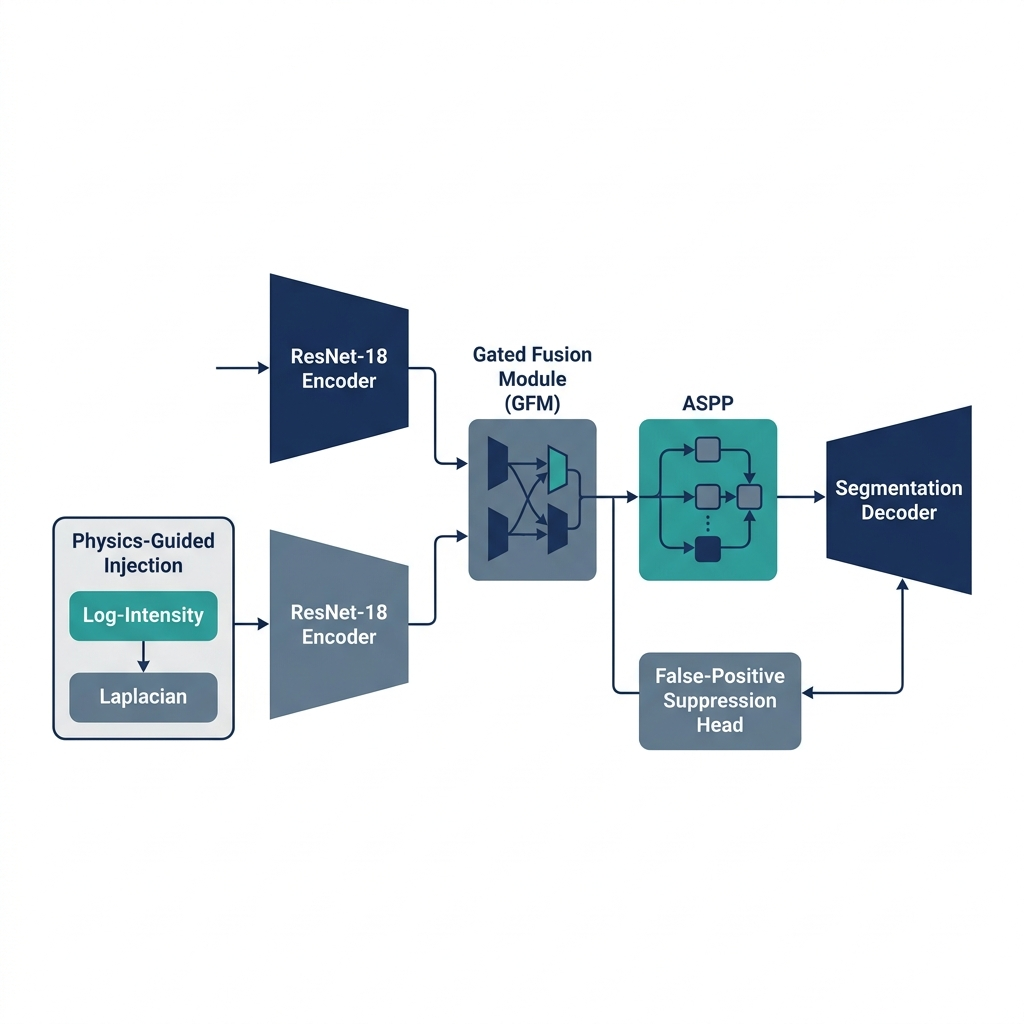
\includegraphics[width=\linewidth]{figures/architecture.png}
\caption{PGDE System Architecture. Rationale: Parallel encoding decoupling prevents spectral spectral glint from suppressing subtle SAR backscatter tokens, while Stage-1 physics injection grounds the latent space before semantic depth. Component: Symmetric Dual-Encoder with Physics-Prior Gating.}
\end{figure}

The framework utilizes symmetric parallel ResNet-18 encoders ($E_{RGB}$, $E_{SAR}$). \textit{Rationale:} Symmetric dual-streams are necessary to isolate modality-specific noise. SAR speckle follows a multiplicative distribution while RGB glint is additive; a single backbone cannot effectively learn suppressive weights for both simultaneously.

Feature extraction at Stage 1 integrates the physical transform $\Phi$:
\begin{align}
    F^{stage1}_{SAR} &= H_{SAR}(X_{SAR}) + \Phi(X_{SAR}) \\
    F^{stage1}_{RGB} &= H_{RGB}(X_{RGB})
\end{align}
\textit{Rationale:} Injecting physics-priors at Stage 1 anchors the neural manifold to structural boundaries before high-level residual blocks distort the gradients.

\subsection{Physics-Guided Feature Injection}
We resolve the \textit{Intensity-Damping Paradox} through two specific transforms derived from the SAR intensity $I$:

\textbf{1. Adaptive Log-Intensity Mapping:}
\begin{equation}
\mathcal{L}(I) = \frac{255.0}{\log(1 + I_{max})} \cdot \log(1 + I) 
\end{equation}
\textit{Rationale:} This transform compresses high-dynamic range sea-clutter while stretching the contrast of dark-spot filaments, enabling the encoder to detect spills in heterogeneous sea states.

\textbf{2. Laplacian Structural Prior:}
\begin{equation}
\mathcal{V}(I) = \left| \frac{\partial^2 I}{\partial x^2} + \frac{\partial^2 I}{\partial y^2} \right|
\end{equation}
\textit{Rationale:} Mechanical crude oil spills exhibit sharp, viscosity-driven boundary damping. The Laplacian isolates these second-order derivatives, providing a structural signature that biogenic lookalikes typically lack.

\subsection{Multiscale Atrous Spatial Pyramid Pooling (ASPP)}
\textit{Rationale:} Global contexts are required to differentiate widespread oil plumes from localized boat-wakes. ASPP utilizes dilated convolutions to capture multiscale features without the spatial resolution loss inherent in standard downsampling.

\subsection{Dynamic Gated Fusion Module (GFM)}
Integration is governed by a learned gating weight $\alpha$:
\begin{equation}
F_{\text{fused}} = \alpha(F_{\text{SAR}}) \odot F_{\text{SAR}} + (1 - \alpha(F_{\text{SAR}})) \odot F_{\text{RGB}}
\end{equation}
\textit{Rationale:} GGFM allows the network to adaptively ignore RGB channels during high-glint conditions, prioritizing the structural stability of the SAR tokens.

\subsection{Auxiliary False-Positive Suppression Head}
The operational reliability is enforced by an auxiliary classification head $\Psi$ operating on the bottleneck $Z$:
\begin{equation}
y_{\text{fp}} = \Psi(Z_{\text{bottleneck}}) = \sigma(W_2 \cdot \text{ReLU}(W_1 Z + b_1) + b_2)
\end{equation}
The final segmented output $P_{\text{final}}$ is computed as:
\begin{equation}
P_{\text{final}} = P_{\text{raw}} \cdot [ \text{sigmoid}(-\gamma \cdot y_{\text{fp}}) ]
\end{equation}
\textit{Rationale:} To minimize the $O(10^5)$ USD cost of operational false alarms, the system must prioritize precision. The suppression head gates the segmentation output, ensuring that alerts only propagate for verified petroleum signatures.

The Post-Inference Environmental Constraint Layer (PIECL) operates strictly as a post-inference module and does not influence model training. This structural separation ensures that all reported performance metrics reflect the fundamental learned model capacity, while high operational robustness is achieved through domain-constrained filtering during the deployment phase.
